\chapter{Evaluation}
In this chapter, we analyse the performance impact of the IOMMU, directly comparing it to the physical address approach. We will not be comparing the performance of memory allocation and mapping as in high throughput applications it should be negligable. The main focus lies on the IOMMU itself and how it performs with different page sizes.

\section{Setup}
We benchmark the performance of the driver on two systems.
Both systems run Ubuntu 23.10.

\begin{table}
    \centering
    \begin{tabular}{lllrll}
        \textbf{CPU}                        & \textbf{Year}                         & \textbf{Arch.}  & \textbf{Memory} & \textbf{NVMe} & \textbf{Count} \\
        \toprule

        \multirow{2}{*}{Intel Xeon E5-2660} & \multirow{2}{*}{2012}                 &
        \multirow{2}{*}{Sandy Bridge}       & \multirow{2}{*}{\SI{256}{\giga\byte}} & Samsung Evo 970 &
        \multirow{2}{*}{1}                                                                                                                               \\
                                            &                                       &                 &                 & Plus NVMe     &                \\ \hline

        \multirow{2}{*}{AMD Epyc ...}       & \multirow{2}{*}{2014}                 &
        \multirow{2}{*}{AMD arch}           & \multirow{2}{*}{\SI{1}{\tera\byte}}   & Samsung PM9A3   &
        \multirow{2}{*}{8}                                                                                                                               \\
                                            &                                       &                 &                 & NVMe          &                \\
        \bottomrule
    \end{tabular}

    \caption{System configurations of servers used for performance analysis.}
    \label{tab:servers}
\end{table}


% IOMMU specs, processor, ...

As Linux as well as our IOMMU supports 4KiB, 2MiB and 1GiB page sizes we will test and analyse how it affects the overall performance.

\section{Overall Latency and Throughput}
First, we will compare the VFIO implementation to the MMIO implementation using latency and throughput tests. In these tests, we repeatedly write/read from a 4KiB buffer in the memory. Each I/O operation uses a 4KiB unit size.

In these tests, we can see that there is practically a negligable amount of overhead. As this test only uses a one page buffer at maximum, the buffer is constantly stored in the IOTLB.

This test uses one buffer from which the NVMe driver reads/writes to. This buffer and the Queues can fit on the IOTLB. Fetching addresses from the IOTLB is very efficient and thus, no significant performance impact occurs.

\begin{figure}
    \centering
    \subcaptionbox {Random write} {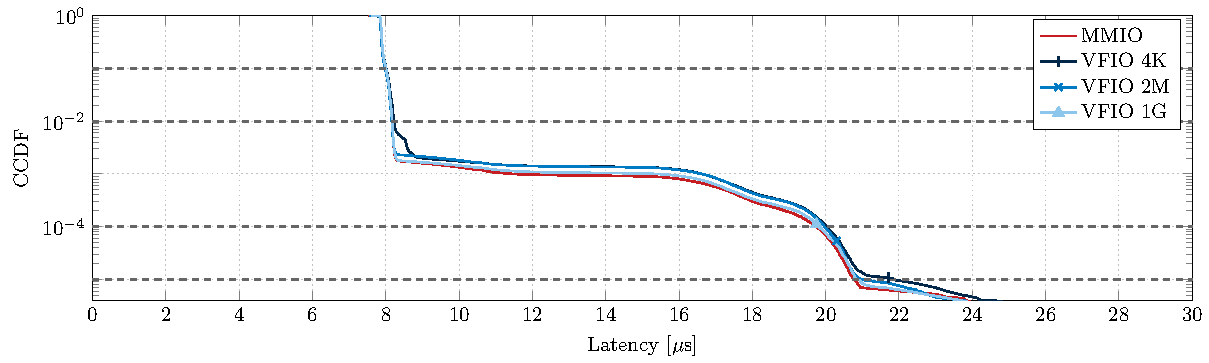
\includegraphics[width=\textwidth]{figures/latency_ccdf_write} \label{fig:ccdf-write}}
    \subcaptionbox {Random read} {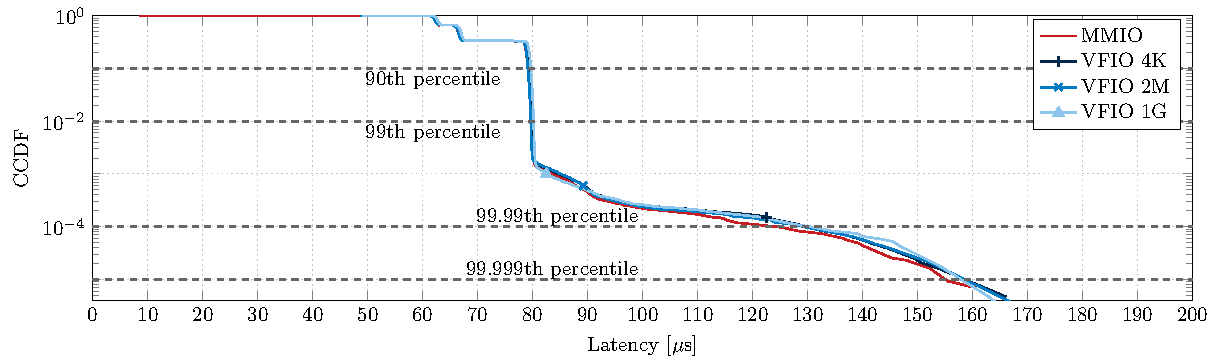
\includegraphics[width=\textwidth]{figures/latency_ccdf_read} \label{fig:ccdf-read}}
    \caption{Tail latencies}
    \label{fig:ccdf}
\end{figure}

\begin{figure}
    \centering
    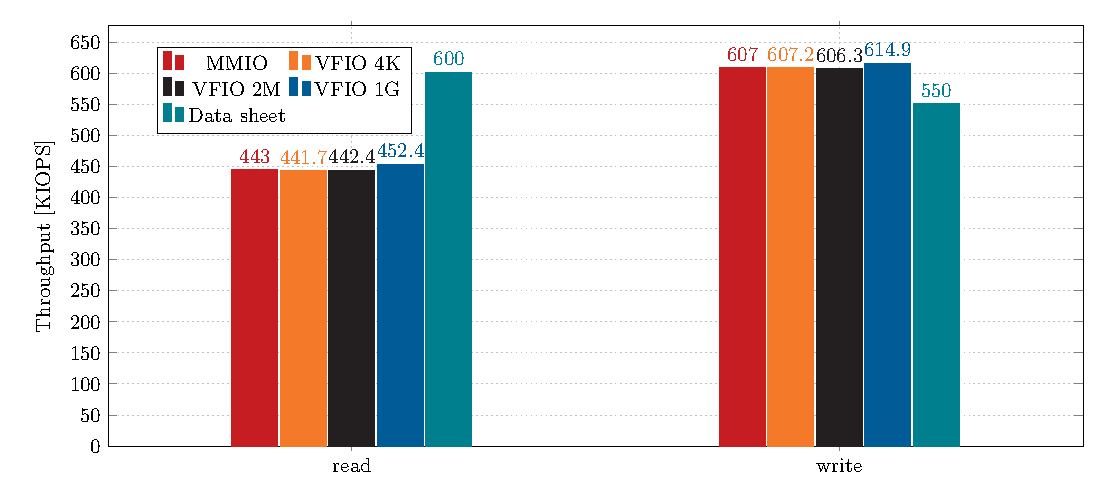
\includegraphics[width=\textwidth]{figures/throughputqd32t1singlepage}
    \caption{Write and Read Operations with queue depth 32 and 4 threads}
    \label{fig:iopsq32t1sp}
\end{figure}

\section{IOTLB}
As the size of the IOTLB is not stated in hardware and VT-d specifications, we use a latency test to analyse the behaviour of the IOMMU. We can assume that the IOTLB entry count must be a power of two. In order to isolate the effect of the IOMMU we use the median of 1 Byte random write latencies on the emptied NVMe. We repeatedly Write to a number of pages that is an increasing power of two. Taking the median and comparing them we can figure out where a latency spike occurs and can then derive the IOTLB size. We configure the queues, buffer and prp-list to each take up one page, resulting in 6 allocated pages before the actual workload. This test is done using without the IOMMU with 2MiB pages and the IOMMU with 4KiB, 2MiB and 1GiB pages.
In order to test 1GiB pages, we first need to increase the ulimit settings, as memlock limits the amount of locked-in-memory address space.
On the resulting graph \autoref{fig:med-ps} we can observe a performance spike of around 300 nanoseconds for each write between 128 and 256 allocated pages. In the case of 4KiB pages, this is a memory size of only 512 KiB.

\begin{figure}
    \centering
    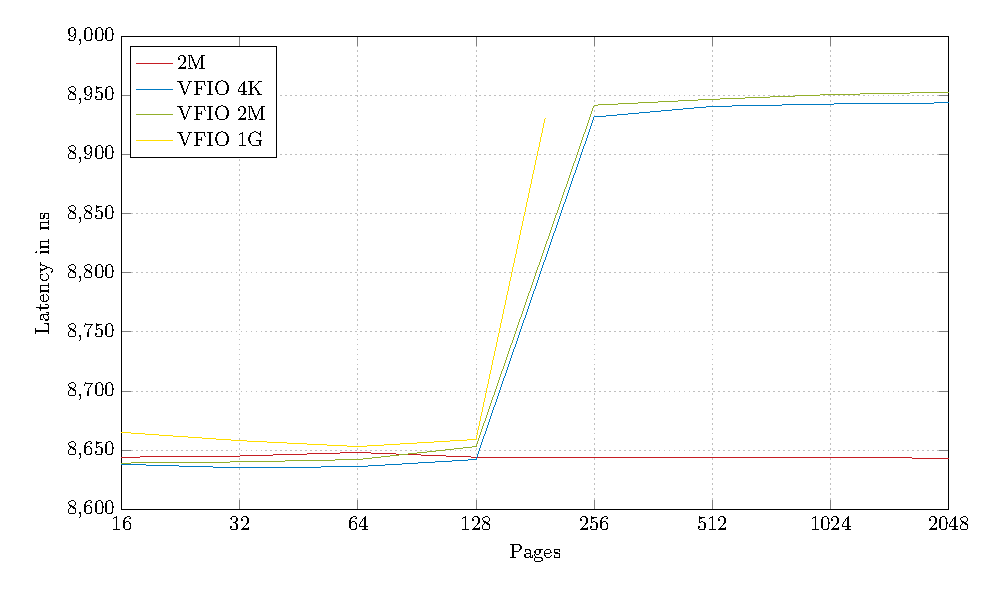
\includegraphics[width=\textwidth]{figures/pagesizemedians}
    \caption{Pagesize Medians}
    \label{fig:med-ps}
\end{figure}

Using multithreaded random writes with queue deoth, we can see up to 10\% less performance using 4KiB pages. As we use a buffer of 2MiB, the Vfio 2MiB performance drops at 64 threads.

\begin{figure}
    \centering
    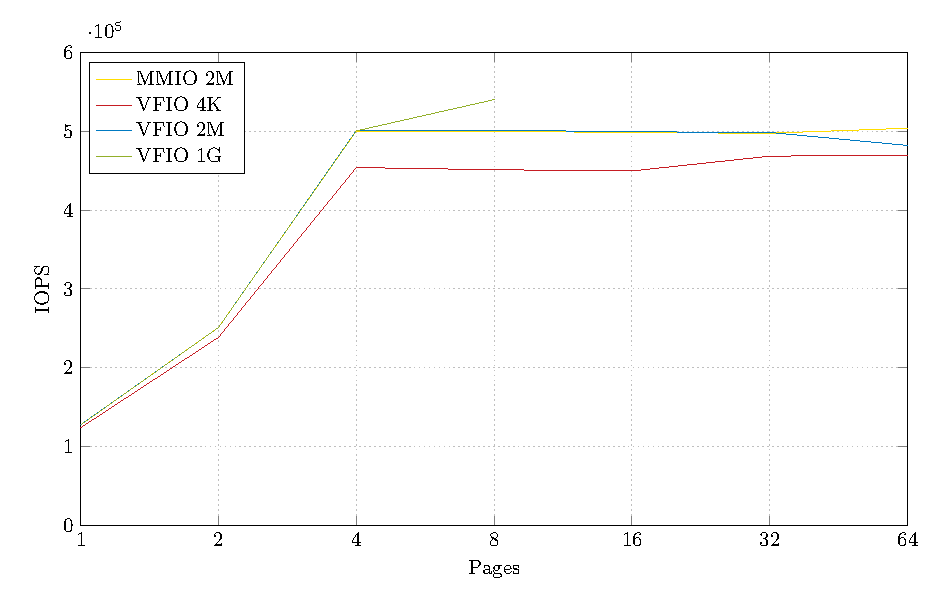
\includegraphics[width=\textwidth]{figures/qd1tnrandwrite}
    \caption{QD1 Random Write Throughput with multithreading}
    \label{fig:qd1tn}
\end{figure}



\section{IOMMU modes}